\section{Data sets and triggers}
%%%%%%%%%%%%%%%%%%%%%%%%%%%%%%%%%%%%%%%%%%%%%%%%%%%%%%%%%%%%%%%%%%%%%%
\label{sec:Datasets}

%-------------------------------------------------------------------------------
%\subsection{Data sets and triggers\label{subsec:Datasets}}
The data set used for this analysis corresponds to 19.4\ifb of proton-proton collisions at $\sqrt{s}=8$\TeV, collected by the CMS detector during 2012.
Only data corresponding to good data taking quality are considered.

Events are required to fire one of the unprescaled single-electron, single-muon or muon-electron triggers. Due the rather high LHC instantaneous luminosity the single-lepton triggers must have high HLT \pt thresholds, otherwise the rate of these triggers would be too large to be sustained. The double-lepton triggers allow to lower down the \pt thresholds while keeping a sustainable trigger rate, thus maintaining a good sensitivity to the Higgs boson signal, for which the lepton \pt can be rather small.
A brief overview of the HLT \pt criteria on the leptons
is given in Table~\ref{tab:trigger}. While the HLT lepton \pt thresholds of 17 and 8 \GeV for the double
lepton triggers accommodate the offline lepton \pt selection of 20 and 10 \GeV, the higher \pt thresholds
in the single lepton triggers help partially recovering double lepton trigger inefficiencies
as a high \pt lepton is on average expected due to the kinematic of the Higgs decay. 

\begin{table}[h]
\begin{center}
\caption{Transverse momentum thresholds applied in the lepton triggers at the HLT level. 
         Double set of thresholds indicates the thresholds for each leg of the double lepton triggers.}
\begin{tabular}{ccc}
\toprule
Trigger path       & Threshold \\
\midrule
Single electron    & $\pt > 27 $ \GeV         \\  
Single muon        & $\pt > 24 $ \GeV         \\ 
Muon-Electron      & $\pt > 17$ and $8 $ \GeV         \\ 
Electron-Muon      & $\pt > 17$ and $8 $ \GeV         \\ 
\bottomrule
\end{tabular}
\label{tab:trigger} 
\end{center}
\end{table}

The trigger is not simulated in MC samples but the combined trigger efficiency
is estimated from data and applied as a weight to all simulated events, as described in Sec.~\ref{sec:trigeff}.
% The trigger efficiency for single and double lepton triggers is calculated using a Tag and Probe technique separately for muons and electrons, in bins of $\eta$ and \pt.
%%%%%%%%%%%%%%%%%%%%
%%%%%%%%%%%%%%%%%%%% 

%SPOSTATO IN CAP. 2
%The Tag and Probe method uses a known mass resonance (e.g. $J/\Psi$, Z) to select particles of the desired type, and probe the efficiency of a particular selection criterion on these particles. In general the ``tag'' is an object that passes a set of very
%tight selection criteria designed to isolate the required particle type. Tags are often referred
%to as a “golden” electrons or muons and the fake rate for passing tag selection criteria should
%be very small. A generic set of the desired particle type (i.e. with potentially very loose selection criteria) known as ``probes'' is selected by pairing these objects with tags such that the
%invariant mass of the combination is consistent with the mass of the resonance. Combinatoric
%backgrounds may be eliminated through any of a variety of background subtraction methods
%such as fitting, or sideband subtraction. The definition of the probe objects depend on the
%specifics of the selection criterion being examined. The simple expression to get the efficiency $\epsilon$
%as a function of \pt and $\eta$ is given below:
%
%\begin{equation}
%\epsilon(\pt,\eta) = \frac{ N^\mathrm{probe}_\mathrm{pass}}{N^\mathrm{probe}_\mathrm{pass} + N^\mathrm{probe}_\mathrm{fail}}
%\end{equation}
%%%%%%%%%%%%%%%%%%%%%
%%%%%%%%%%%%%%%%%%%%%
%For double lepton triggers the efficiency is calculated separately for each leg of the trigger and then combined together. In the calculation the efficiencies of the two trigger legs are considered as independent, given that the correlations are very small. The combined efficiency is then used as a kinematics-dependent weight to be applied on top of simulated events.
%
%The event efficiency $\epsilon_\mathrm{ev}$ for an event with two leptons to pass the single lepton trigger is given by the following formula:
%
%\begin{equation}\label{eq:single_trigg}
%\epsilon_\mathrm{ev} = 1 - (1-\epsilon_{S,\ell1})\cdot(1-\epsilon_{S,\ell2})\quad,
%\end{equation}
%
%where $\epsilon_{S,\ell1}$ and $\epsilon_{S,\ell2}$ are the efficiencies for the leading and subleading lepton to pass the single lepton trigger. In other words, the dilepton event passes the single lepton trigger if either one of the two leptons passes the single lepton trigger, excluding the cases for which both leptons pass the trigger. For double lepton triggers, the event efficiency can be written as:
%
%\begin{equation}\label{eq:double_trigg}
%\epsilon_\mathrm{ev}  = \epsilon_{D,\ell1}^\mathrm{lead} \cdot \epsilon_{D,\ell2}^\mathrm{trail} + (  1 -  \epsilon_{D,\ell1}^\mathrm{lead} \cdot \epsilon_{D,\ell2}^\mathrm{trail})\cdot\epsilon_{D,\ell1}^\mathrm{trail} \cdot \epsilon_{D,\ell2}^\mathrm{lead} \quad,
%\end{equation}
%
%where $\epsilon_{D,\ell1}^{\mathrm{lead}(trail)}$ is the efficiency of the first lepton to pass the leading (trailing) leg of the double lepton trigger, and $\epsilon_{D,\ell2}^{\mathrm{lead}(trail)}$ is the efficiency of the second lepton to pass the leading (trailing) leg of the double lepton trigger. The final event efficiency applied to reweight the events in simulation is given by the boolean OR of the event efficiencies corresponding to the single and double lepton triggers, which, using Eqs.~\eqref{eq:single_trigg} and ~\eqref{eq:double_trigg}, can be written as:
%
%\begin{equation}
%\begin{split}
%\epsilon_\mathrm{ev} & = 1 - (1-\epsilon_{S,\ell1})\cdot(1-\epsilon_{S,\ell2}) + \\
%                     & + (1-\epsilon_{S,\ell1})\cdot(1-\epsilon_{S,\ell2}) \cdot \\
%                     & \cdot [ \epsilon_{D,\ell1}^\mathrm{lead} \cdot \epsilon_{D,\ell2}^\mathrm{trail} + (  1 -  \epsilon_{D,\ell1}^\mathrm{lead} \cdot \epsilon_{D,\ell2}^\mathrm{trail})\cdot\epsilon_{D,\ell1}^\mathrm{trail} \cdot \epsilon_{D,\ell2}^\mathrm{lead} ] \quad.
%\end{split}
%\end{equation}
%
%The term that multiplies the double lepton trigger event efficiency is needed to ensure that the events passing the double lepton trigger do not pass also the single lepton trigger.


%-------------------------------------------------------------------------------
\section{Monte Carlo samples\label{subsec:MC}}

Several Monte Carlo event generators are used to simulate the signal and background processes:
\begin{itemize}
\item the first version of the \textsc{Powheg} program (\textsc{Powheg V1}) provides event samples for the \hww signal
for the ggH and VBF production mechanisms, as well as \ttbar and tW processes~\cite{Alioli:2011as}, with NLO accuracy;
\item the VH process is simulated using \textsc{pythia 6.426}~\cite{Sjostrand:2006za};
\item the $\mathrm{qq} \to \mathrm{W^{+}W^{-}}$, Drell-Yan, ZZ, WZ, W$\gamma$, W$\gamma^*$, tri-bosons and W+jets processes are generated using
the \textsc{Madgraph 5.1.3} event generator;
\item the gg$\to \mathrm{W^{+}W^{-}}$ process is generated using the \textsc{gg2ww} 3.1 generator ~\cite{Binoth:2006mf} and its cross section is scaled to the approximate NLO prediction~\cite{Bonvini:2013jha,Passarino:2013bha}.
\end{itemize}
For samples generated at leading-order (LO) accuracy in perturbative QCD, the \textsc{cteq6l}~\cite{Lai:2010nw} set of parton distribution functions
(PDF) is used, while \textsc{ct10}~\cite{Lai:2010vv} is used for next-to-leading order (NLO) ones.
Cross section calculations at next-to-next-to-leading order (NNLO) are used for the \hww process~\cite{Dittmaier:2011ti}.
The $\hww$ process simulation is reweighted so that the \pth spectrum and inclusive production cross section closely match the SM calculations that have NNLO+NNLL QCD accuracy in the description of the Higgs boson inclusive production, in accordance with the LHC Higgs Cross Section Working Group recommendations~\cite{Heinemeyer:2013tqa}.
The reweighting of the \pth spectrum is achieved by tuning the \textsc{Powheg} generator, as described in detail in Ref.~\cite{Alioli:2010xd}.
Cross sections computed with NLO QCD accuracy are used for the background processes~\cite{Heinemeyer:2013tqa}.
The contribution of the \ttH production mechanism is checked to be negligible (below 1\%) in the whole \pth spectrum and is not included in the analysis. In Fig.~\ref{fig:signal_comp} the relative fraction of the four production mechanisms is shown for each \pth bin.

\begin{figure}[htb]
\centering
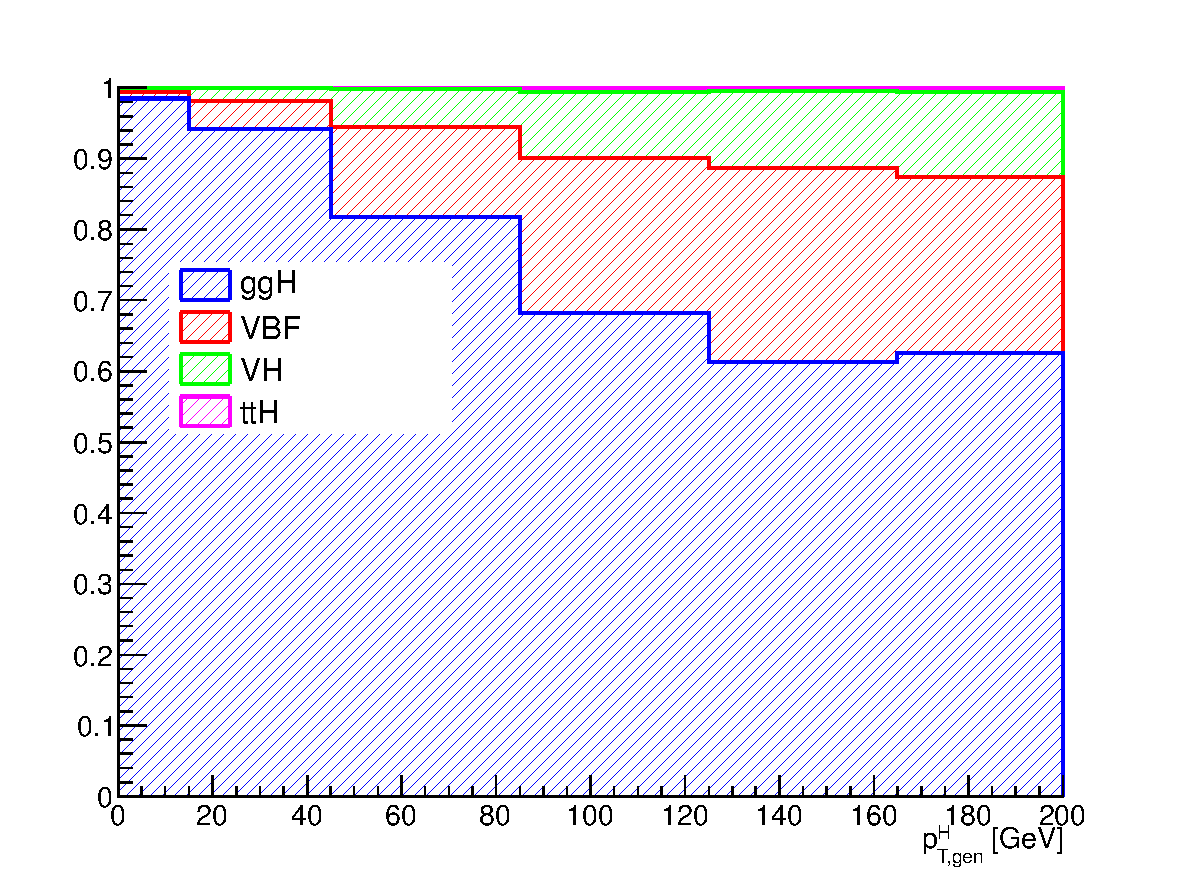
\includegraphics[width=0.7\textwidth]{images/signal_composition_ttH.pdf}
\caption{Relative fraction of ggH, VBF, VH and \ttH in each bin of the Higgs boson transverse momentum.}\label{fig:signal_comp}
\end{figure}

For all processes, the detector response is simulated using a detailed description of the CMS detector, based on the \textsc{Geant4} package~\cite{Agostinelli:2002hh}.

Minimum bias events are superimposed on the simulated events to emulate the additional 
proton-proton interactions per bunch crossing. The pile-up multiplicity in simulated events has been generated poissonianly sampling from a distribution similar to the one expected from data.
The simulated events are reweighted to correct for observed differences between data and simulation in the number of pile-up events, as shown in Fig.~\ref{fig:nvertices}.

\begin{figure}[htb]
\centering
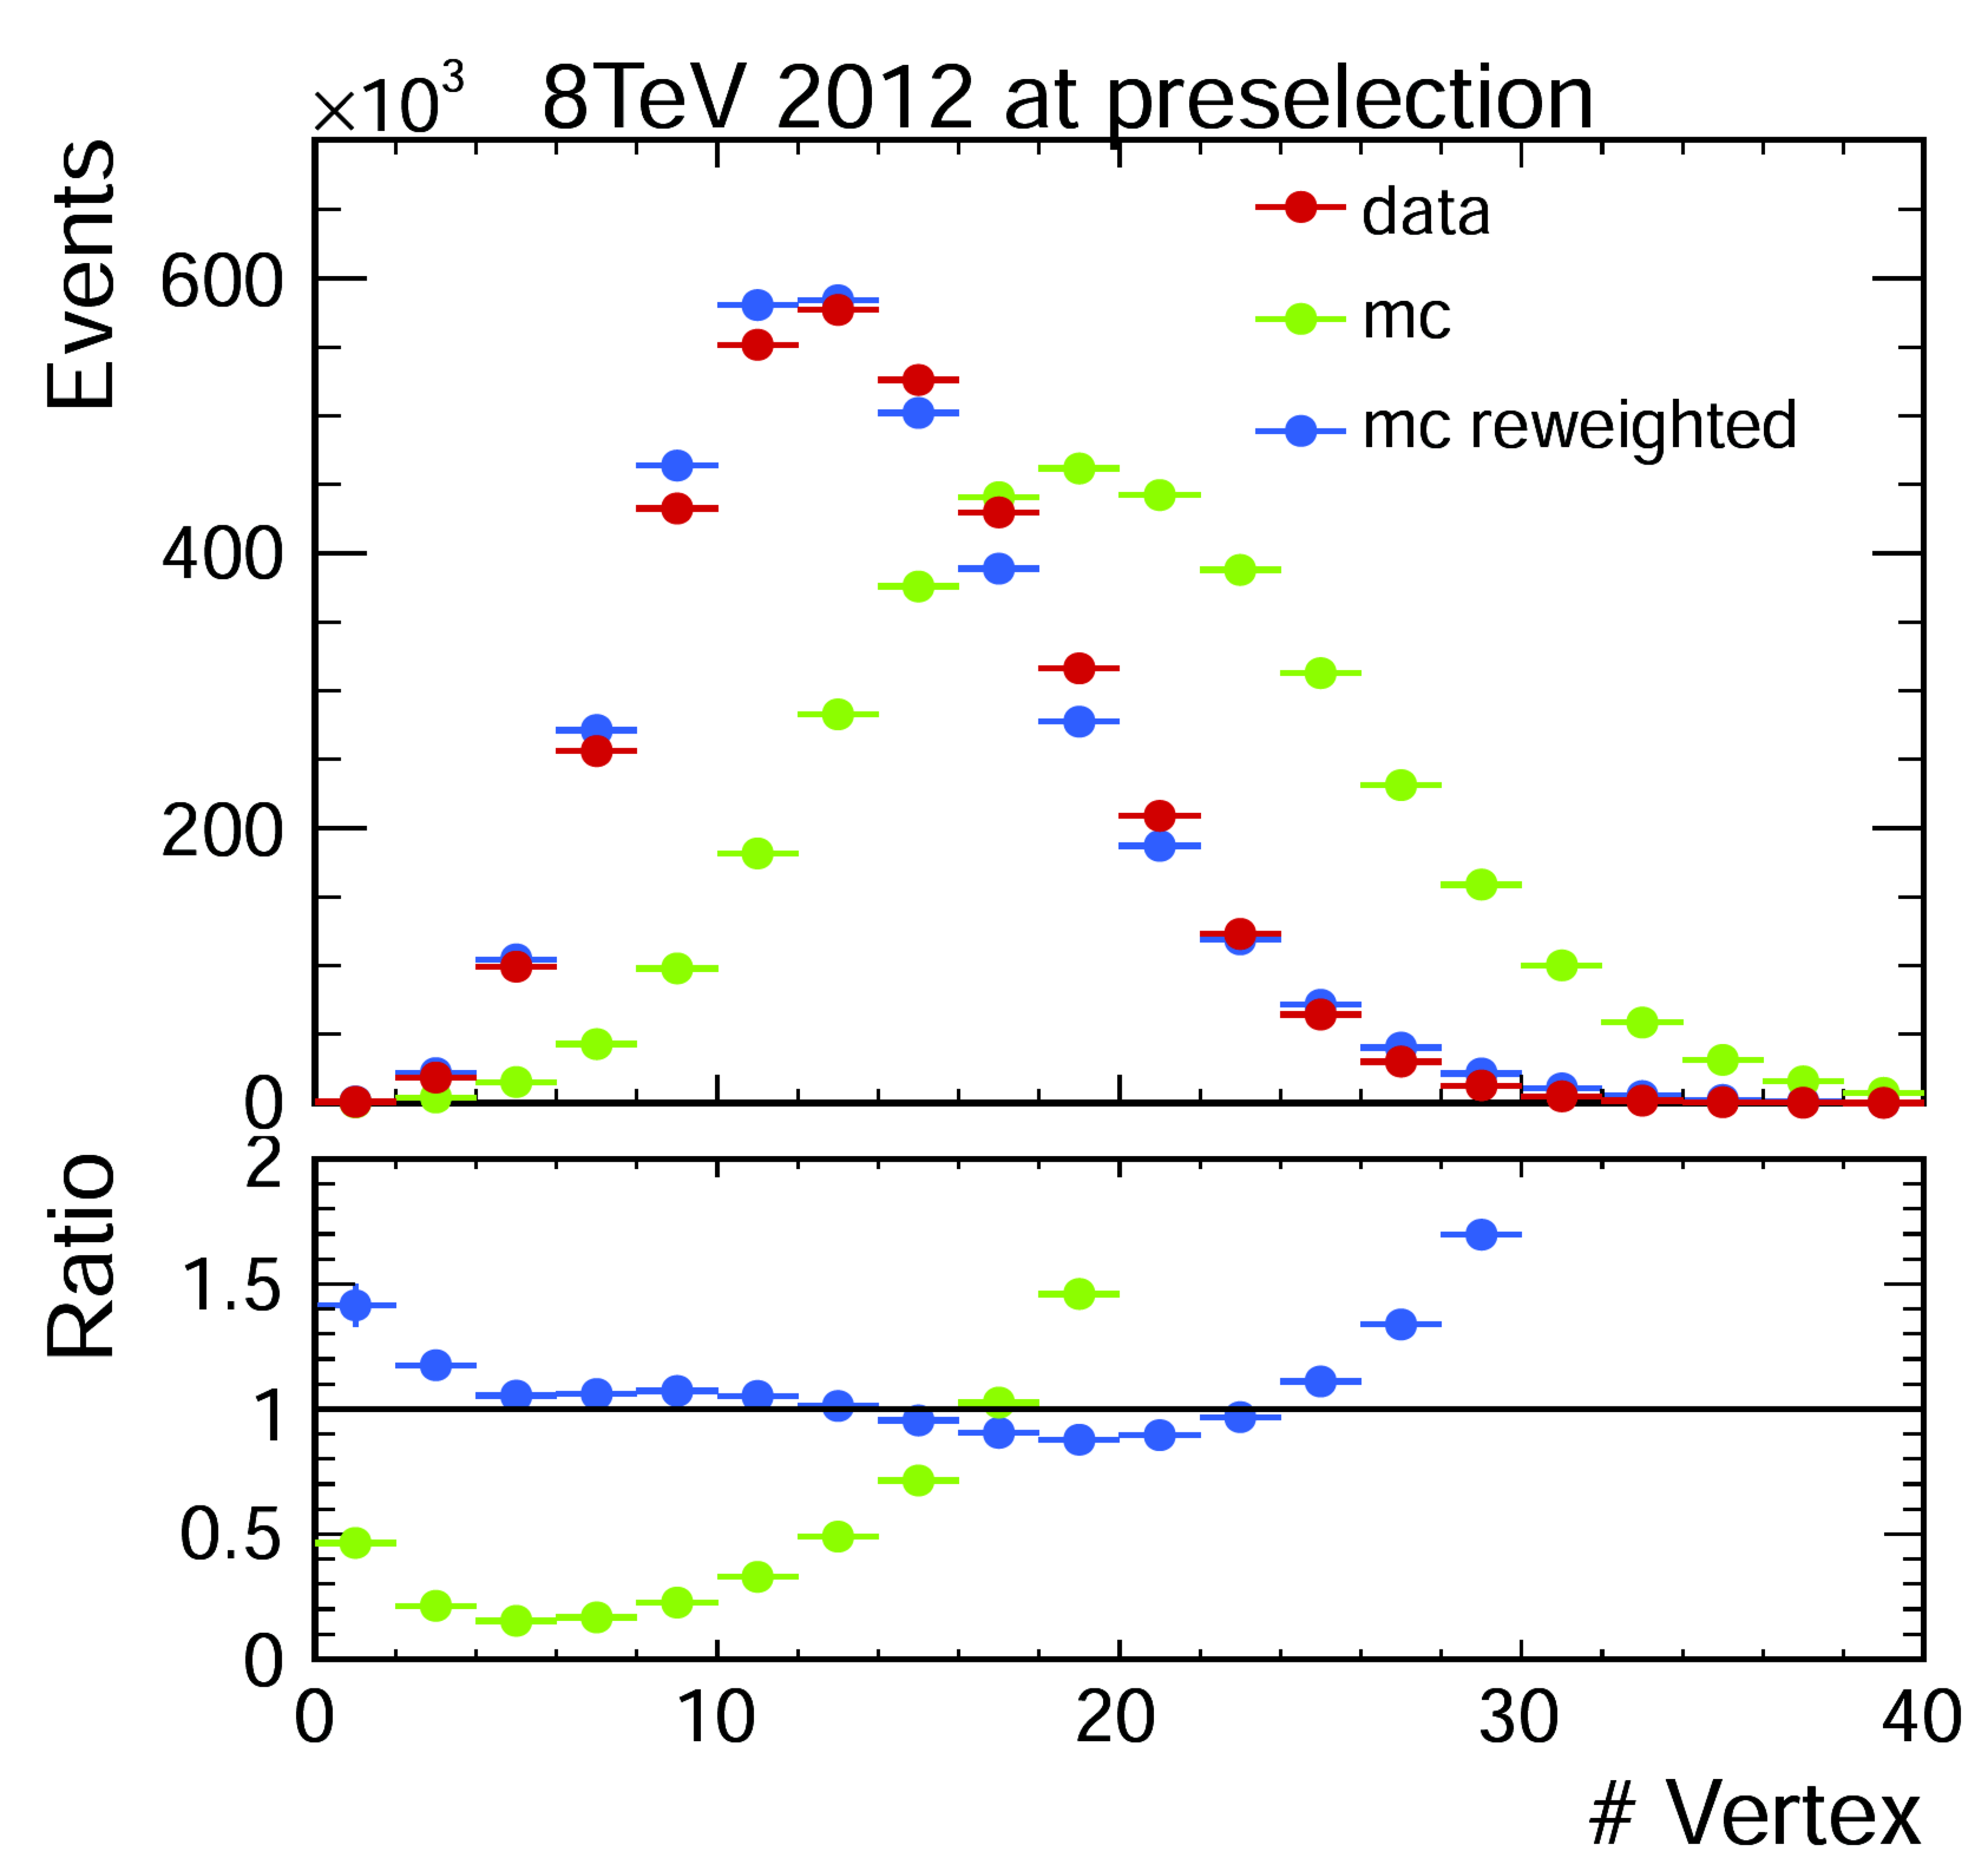
\includegraphics[width=0.7\textwidth]{images/nvertex.pdf}
\caption{Distribution of the number of vertices in data and simulation, before and after applying the pile-up reweighting.}\label{fig:nvertices}
\end{figure}

For the comparison of the measured unfolded spectrum with the theoretical predictions, two additional MC generators are used for simulating the SM Higgs boson production in the ggH process: \textsc{HRes} 2.3~\cite{deFlorian:2012mx,Grazzini:2013mca} and the second version of the \textsc{Powheg} generator (\textsc{Powheg V2})~\cite{Bagnaschi:2011tu}.
\textsc{HRes} is a partonic level MC generator that computes the SM Higgs
boson cross section at NNLO accuracy in QCD and performs the NNLL
resummation of soft-gluon effects at small \pt. The central predictions of
\textsc{HRes} are obtained including the top and bottom quark mass contribution to
the gluon fusion loop, fixing the renormalization and factorization scale central values at a Higgs boson mass of 125\GeV. The cross section normalization is scaled, to take into account electroweak corrections (by a factor of 1.05) and effects of threshold resummation (by a factor of 1.06)~\cite{Actis:2008ug,Catani:2003zt}. The upper and lower bounds of the uncertainties are obtained by scaling up and down both the renormalization and the factorization scales by a factor of two.
The \textsc{Powheg V2} generator is a matrix element based generator that provides a NLO description of the ggH process in association with zero jets, taking into account the finite mass of the bottom and top quarks.
The \textsc{Powheg} prediction is tuned using the \textsc{Powheg} damping factor \textit{hdump} of 104.17~\GeV, in order to match the \pth{} spectrum predicted by \textsc{HRes} in the full phase space. This factor reduces the emission of additional jets in the high \pt regime, and enhances the contribution from the Sudakov form factor in the limit of low \pt.
The \textsc{Powheg} generator is interfaced to the \textsc{JHUGen} generator version 5.2.5~\cite{Gao:2010qx,Bolognesi:2012mm,Anderson:2013afp} for the decay of the Higgs boson to a W boson pair and interfaced with \textsc{Pythia 8}~\cite{Sjostrand:2007gs} for the simulation of parton shower and hadronization effects.
